\chapter{Validazione della convenzione angolare}
\label{app:validazione}

Questa appendice riporta per esteso la verifica riassunta nel
Paragrafo\ref{sec:ch3:angoli}, con i risultati per singolo giunto.

\section{Metodo}
\label{app:val:metodo}

La verifica è stata eseguita sui file del dataset di
laboratorio\cite{vielemeyer2026}, che contengono nello stesso file sia i marker
grezzi sia le uscite del modello clinico Plug-in Gait full body. Per ciascun file
lo strumento svuota gli angoli presenti nella sorgente, li ricalcola dai soli
centri articolari con la convenzione del progetto ed infine confronta le due serie
temporali.

Sono riportati: il valore assoluto della correlazione fra la
serie ricalcolata e quella del modello, le rispettive escursioni ed il residuo,
inteso come scarto quadratico medio fra le due serie punto per punto. La misura
copre 118 prove di due soggetti nelle sei condizioni di pendenza del dataset.

\section{Risultati per giunto}
\label{app:val:risultati}

\begin{table}[htbp]
\centering
\caption{Validazione della convenzione angolare contro un modello clinico
calibrato, su 118 prove. Escursioni e residui in gradi; il residuo è lo scarto
quadratico medio sulla serie temporale. Il caso peggiore è in grassetto.}
\label{tab:app:validazione}
\begin{tabular}{lrrrrr}
\toprule
\textbf{Giunto / piano} & \textbf{File} & $|\mathrm{corr}|$ &
  \textbf{ROM clinico} & \textbf{ROM calcolato} & \textbf{Residuo} \\
\midrule
tronco / frontale     & 118 & 1.000 &  5.1 &  5.1 & 0.0 \\
tronco / sagittale    & 118 & 0.998 &  3.8 &  3.8 & 0.1 \\
tronco / trasverso    & 118 & 0.998 & 11.1 & 11.1 & 0.2 \\
colonna / trasverso   & 118 & 0.998 & 14.6 & 15.7 & 0.3 \\
caviglia sx / sagitt. & 118 & 0.996 & 33.3 & 33.2 & 0.8 \\
caviglia dx / sagitt. & 118 & 0.995 & 34.9 & 34.0 & 0.9 \\
anca sx / sagittale   & 118 & 0.996 & 41.4 & 32.7 & 1.2 \\
anca dx / sagittale   & 118 & 0.997 & 41.9 & 34.4 & 1.2 \\
ginocchio sx / sagitt.& 118 & 0.986 & 68.7 & 69.6 & \textbf{3.2} \\
ginocchio dx / sagitt.& 118 & 0.988 & 67.9 & 67.9 & \textbf{3.2} \\
\bottomrule
\end{tabular}
\end{table}

Il ginocchio è il caso peggiore su entrambi i lati, con un residuo di 3.2 gradi ed
una correlazione di 0.987. In questo caso su un'escursione di
circa 68 gradi, uno scarto quadratico medio di 3.2 gradi corrisponde a meno del
cinque per cento, come si vede nella Figura\ref{fig:app:validazione}.

\begin{figure}[htbp]
\centering
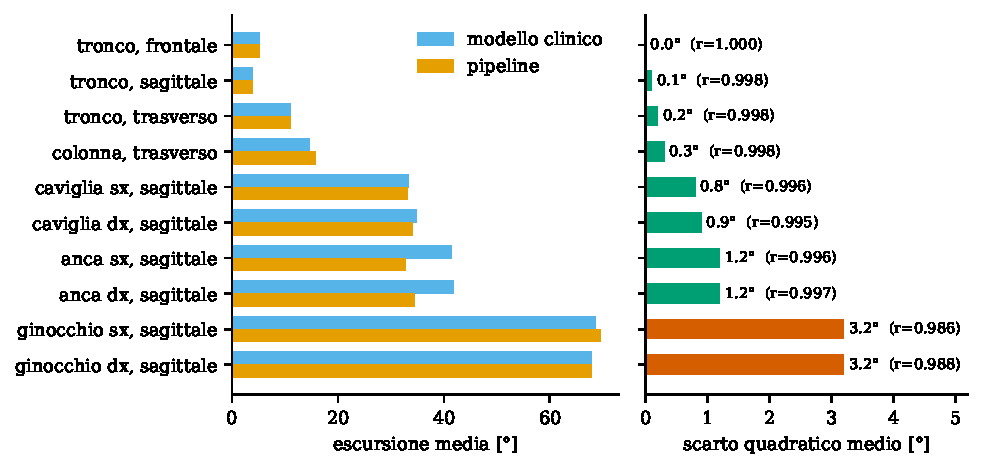
\includegraphics[width=\textwidth]{figures/appendice/app_validazione.pdf}
\caption{Validazione per giunto su 118 prove. A sinistra l'escursione media
secondo il modello clinico e secondo la pipeline; a destra lo scarto quadratico
medio sulla serie temporale, con la correlazione.}
\label{fig:app:validazione}
\end{figure}

